\documentclass[aspectratio=43,11pt]{beamer}
\usetheme{default}
\usepackage[T1]{fontenc}
\usepackage{lmodern}
\usepackage{amsmath}
\usepackage{graphicx}
\usepackage{listings}
\usepackage{xcolor}
\usepackage{hyperref}
\graphicspath{{figures/}}
\definecolor{ink}{HTML}{223247}
\definecolor{accent}{HTML}{500000}
\definecolor{pale}{HTML}{EEF5F6}
\definecolor{codebg}{HTML}{F2F5F7}
\definecolor{lightline}{HTML}{CEDDE2}
\setbeamercolor{normal text}{fg=ink,bg=white}
\setbeamercolor{frametitle}{fg=ink,bg=white}
\setbeamercolor{structure}{fg=accent}
\setbeamercolor{block title}{fg=ink,bg=pale}
\setbeamercolor{block body}{fg=ink,bg=pale}
\setbeamertemplate{navigation symbols}{}
\setbeamertemplate{footline}{\hfill\color{accent}\insertframenumber\kern1.5em\vskip0.7em}
\setbeamertemplate{itemize item}{\color{accent}$\bullet$}
\setbeamerfont{frametitle}{size=\Large,series=\bfseries}
\setbeamersize{text margin left=0.65cm,text margin right=0.65cm}
\lstdefinestyle{python}{language=Python,basicstyle=\ttfamily\small,keywordstyle=\color{accent}\bfseries,commentstyle=\color{black!55},stringstyle=\color{red!55!black},backgroundcolor=\color{codebg},frame=single,rulecolor=\color{lightline},framesep=8pt,breaklines=true,showstringspaces=false,columns=fullflexible,keepspaces=true}
\lstset{style=python}
\newcommand{\stage}[1]{\vspace{-0.5em}{\color{accent}\small\bfseries #1}\par\medskip}
\newcommand{\takeaway}[1]{\medskip\begin{beamercolorbox}[wd=\linewidth,sep=8pt,rounded=false]{block body}#1\end{beamercolorbox}}
\newcommand{\activity}[1]{\medskip\begin{beamercolorbox}[wd=\linewidth,sep=9pt]{block body}#1\end{beamercolorbox}}
\title{Decision Trees and Random Forests}
\subtitle{}
\author{DAEN 300 - Fall 2026}
\date{}

\begin{document}

\begin{frame}
\titlepage
\vspace{-6ex}
\begin{itemize}
\item Explain what a decision tree and random forest do;
\item Spot a tree that is learning noise;
\item Compare models fairly and make a recommendation.
\end{itemize}
\vspace{3ex}
\centering 
\includegraphics[height=1cm]{TAMU_logo.png}
\end{frame}

\begin{frame}{Would you trust this model?}
A decision tree is nearly perfect on its \textbf{training data}.\\
But its prediction regions look jagged and unusually narrow.
\vspace{1em}
\begin{itemize}
\item Is that a good sign, a warning sign, or both?
\item What would you check before trusting it with new data?
\end{itemize}
\activity{Think for 30 seconds, then compare answers with a partner (2 min).}
\end{frame}

\begin{frame}{A tree divides the data into regions}
\centering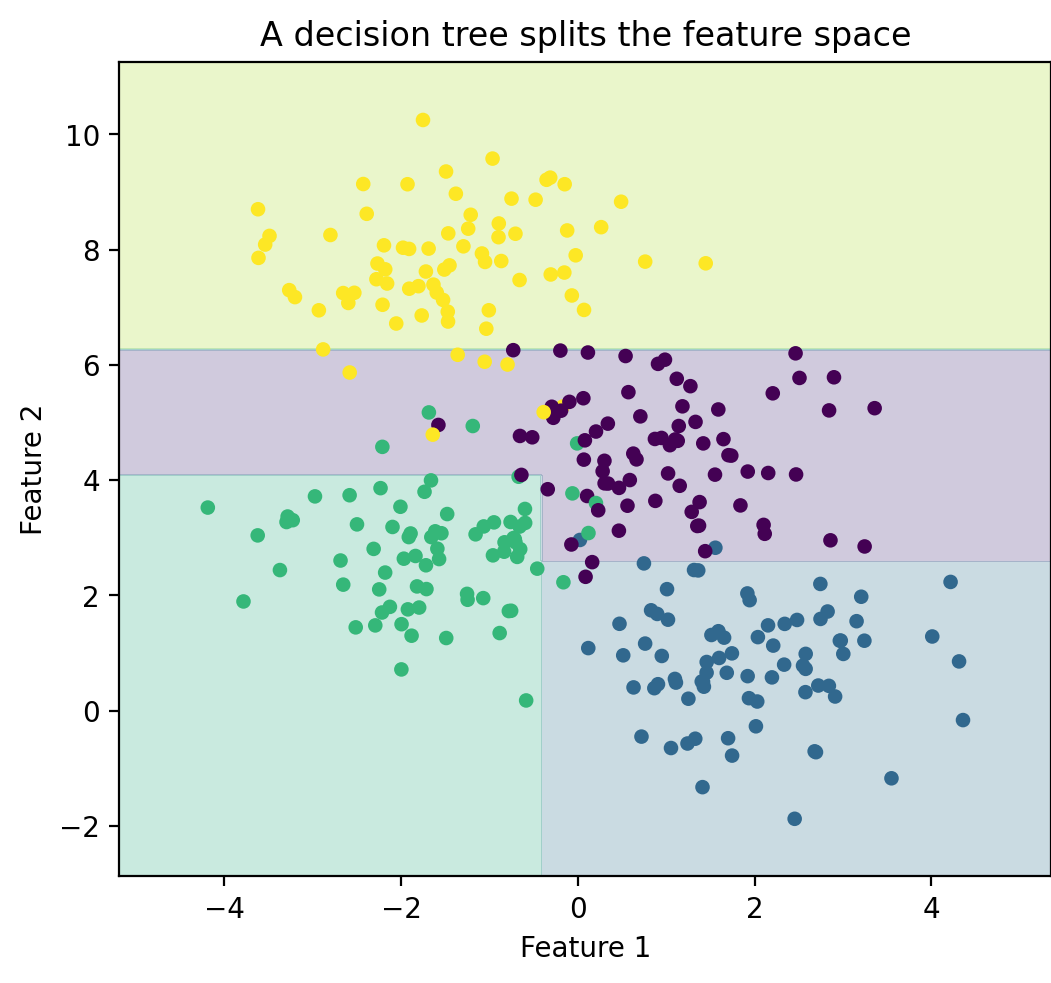
\includegraphics[height=0.7\textheight,keepaspectratio]{tree_regions.png}\par
\vspace{0.3em}\small Each colored area is a prediction.\\
Every straight boundary comes from a simple feature threshold.
\end{frame}

\begin{frame}{The same model is a set of questions}
\centering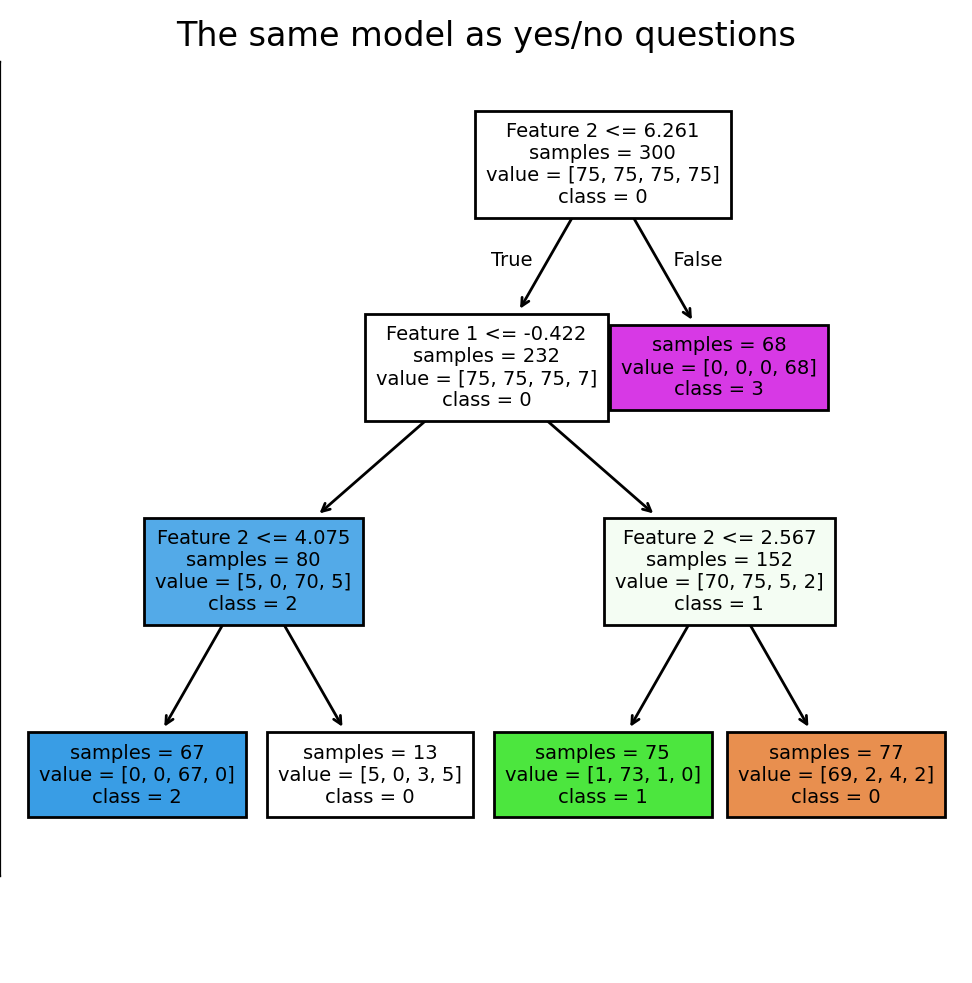
\includegraphics[height=0.7\textheight,keepaspectratio]{tree_questions.png}\par
\vspace{0.3em}\small Follow a path from top to bottom: the final leaf tells us the predicted class.
\end{frame}

\begin{frame}{Why deeper is not always better}
A shallow tree learns broad patterns. A very deep tree can keep splitting until it fits small quirks in the training sample.
\vspace{0.8em}
\begin{itemize}
\item \textbf{Underfitting:} misses important patterns.
\item \textbf{Overfitting:} learns noise that may not repeat.
\item \textbf{Generalization:} works well on new observations.
\end{itemize}
\takeaway{The model with the highest training score is not always the best model for new data.}
\end{frame}

\begin{frame}[fragile]{Try different tree depths}
\begin{lstlisting}
from sklearn.datasets import make_blobs
from sklearn.model_selection import train_test_split
from sklearn.tree import DecisionTreeClassifier

X, y = make_blobs(n_samples=300, centers=4,
                  random_state=0, cluster_std=1.0)
Xtr, Xte, ytr, yte = train_test_split(
    X, y, test_size=.30, stratify=y, random_state=42)

for depth in [2, 5, None]:
    tree = DecisionTreeClassifier(
        max_depth=depth, random_state=0)
    tree.fit(Xtr, ytr)
    print(depth, tree.score(Xtr, ytr),
          tree.score(Xte, yte))
\end{lstlisting}
\end{frame}

\begin{frame}{What did the depth experiment show?}
Compare the training and test accuracy for three tree depths.
\vspace{1em}
\begin{itemize}
\item Which tree had the strongest training score?
\item Did it also have the strongest test score?
\item Which model would you trust more on unseen data?
\end{itemize}
\activity{Write a two-sentence interpretation with your partner (3 min).}
\end{frame}

\begin{frame}{How could we make trees more reliable?}
Imagine asking many slightly different decision trees to classify the same new point.
\par \vspace{1em}
Would their combined answer be \textbf{more stable}, \textbf{less stable}, or \textbf{about the same} as one tree?
\par
\activity{Make a prediction and explain your reasoning.\\
We will check it next.}
\end{frame}

\begin{frame}{One forest, many different boundaries}
\centering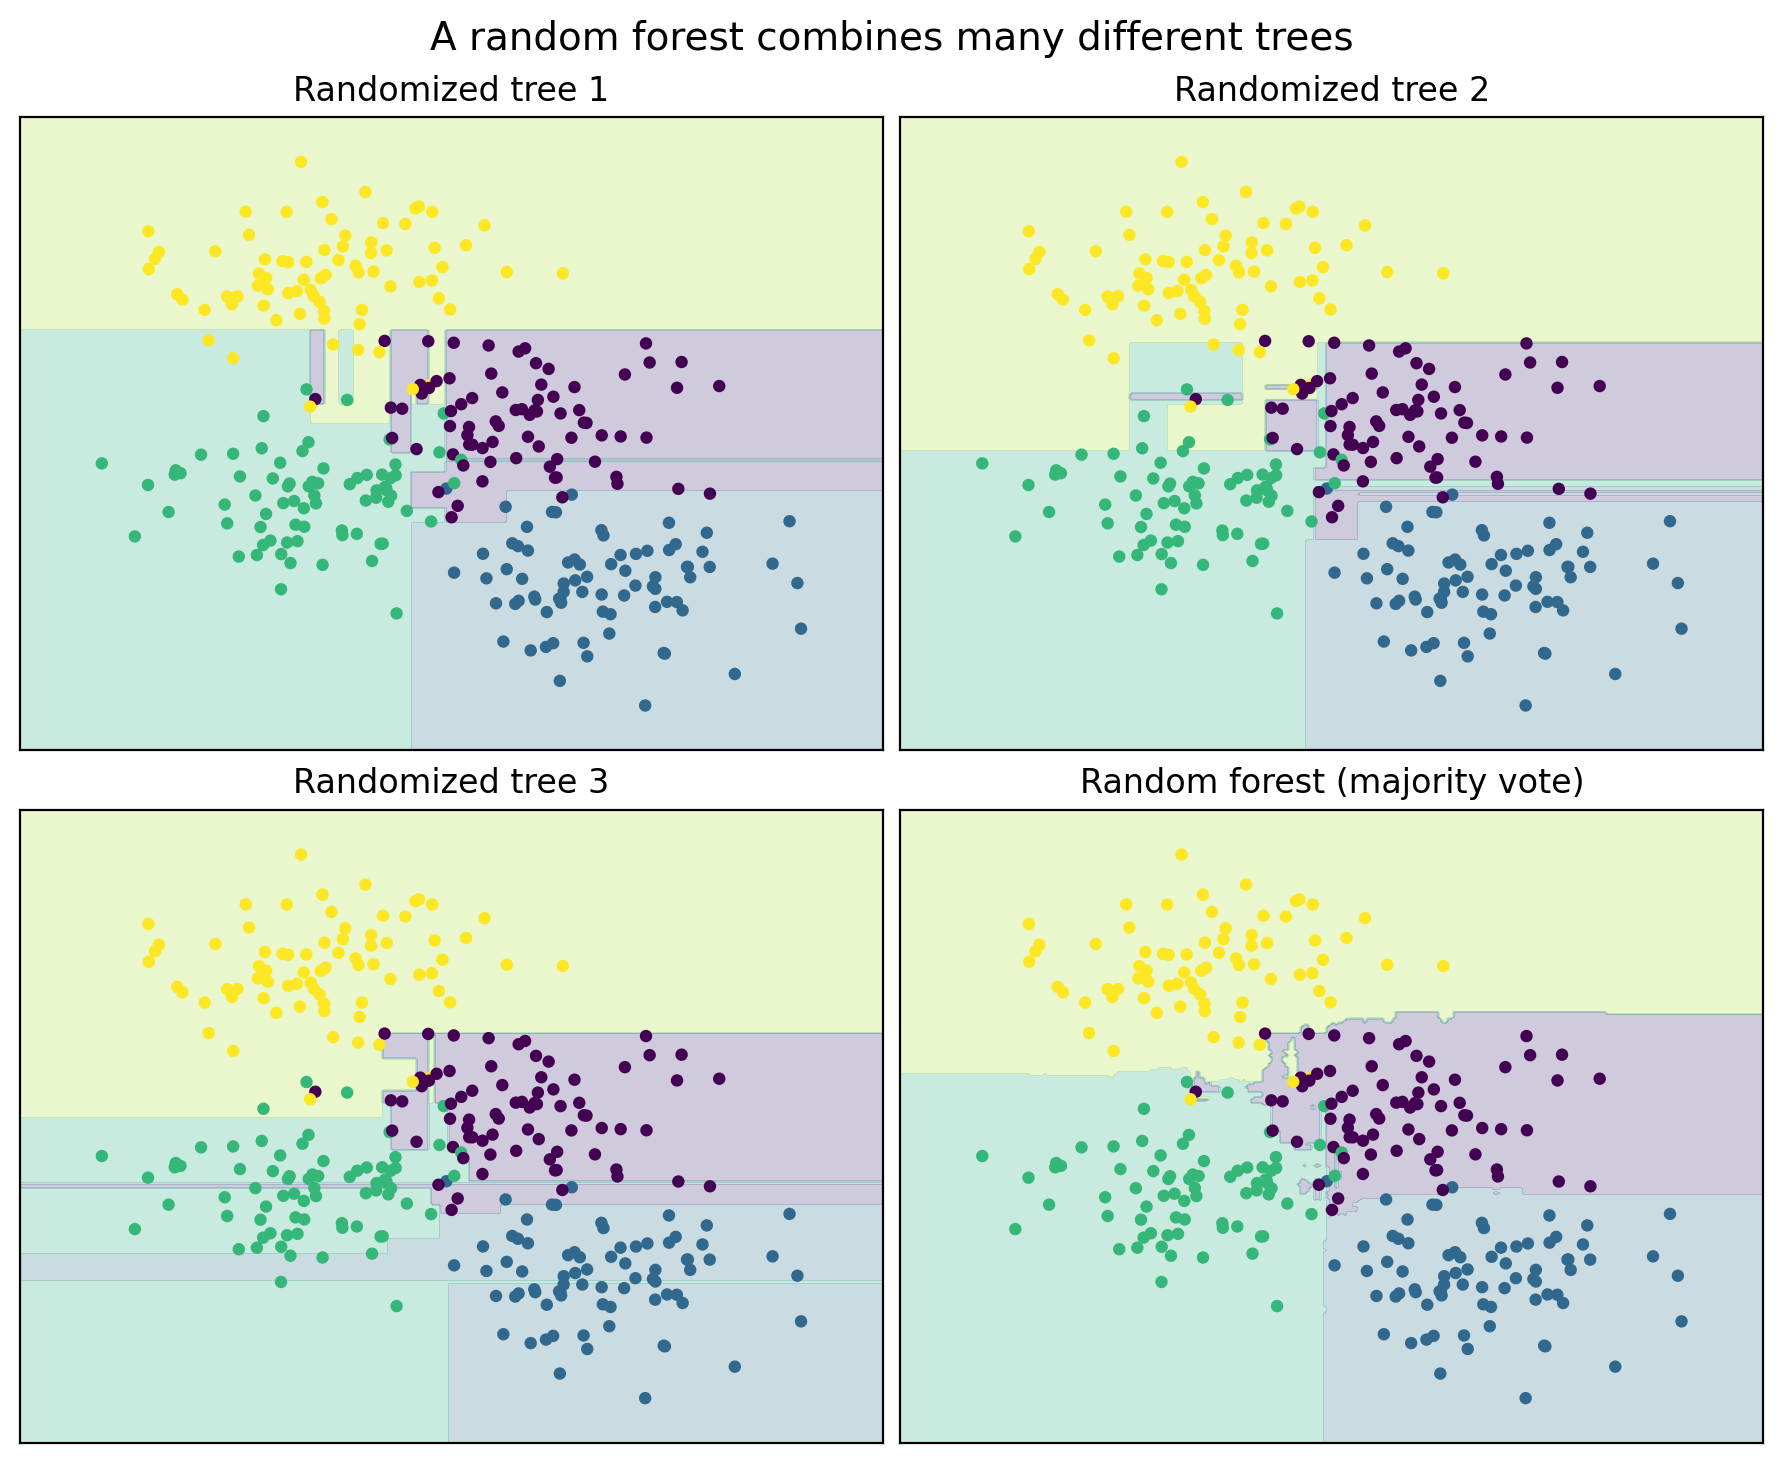
\includegraphics[height=0.67\textheight,keepaspectratio]{random_forest_concept.png}\par
\small The trees disagree in some places.\\
Their combined prediction tends to be less sensitive to individual quirks.
\end{frame}

\begin{frame}{What changes from tree to forest?}
A \textbf{random forest} trains many decision trees and combines their outputs.
\vspace{0.7em}
\begin{itemize}
\item Each tree sees a resampled training set (\textbf{bagging}).
\item At each split, it considers a random subset of features.
\item In classification, the forest combines class votes.
\item In regression, it averages numeric predictions.
\end{itemize}
\takeaway{The useful ingredient is diversity:\\different trees make different mistakes.}
\end{frame}

\begin{frame}{Let the trees vote}
\begin{center}\LARGE A \quad B \quad A \quad A \quad B\end{center}
\vspace{1em}
Five trees classify the same observation. What does the forest predict?
\vspace{0.7em}
\begin{itemize}
\item Which label wins the vote?
\item What share of trees support that label?
\item Why would five identical trees be less useful?
\end{itemize}
\takeaway{The vote is A (3 out of 5 trees).\\
Vote share is not necessarily a calibrated probability.}
\end{frame}

\begin{frame}[fragile]{Compare a tree and a forest}
\begin{lstlisting}
from sklearn.ensemble import RandomForestClassifier

models = {
    "tree": DecisionTreeClassifier(random_state=0),
    "forest": RandomForestClassifier(
        n_estimators=100, random_state=0)
}

for name, model in models.items():
    model.fit(Xtr, ytr)
    print(name, "train:", model.score(Xtr, ytr),
          "test:", model.score(Xte, yte))
\end{lstlisting}
\activity{Which model generalizes better on this split?\\
Do not assume the forest must win.}
\end{frame}

\begin{frame}{Forests can predict numbers, too}
\centering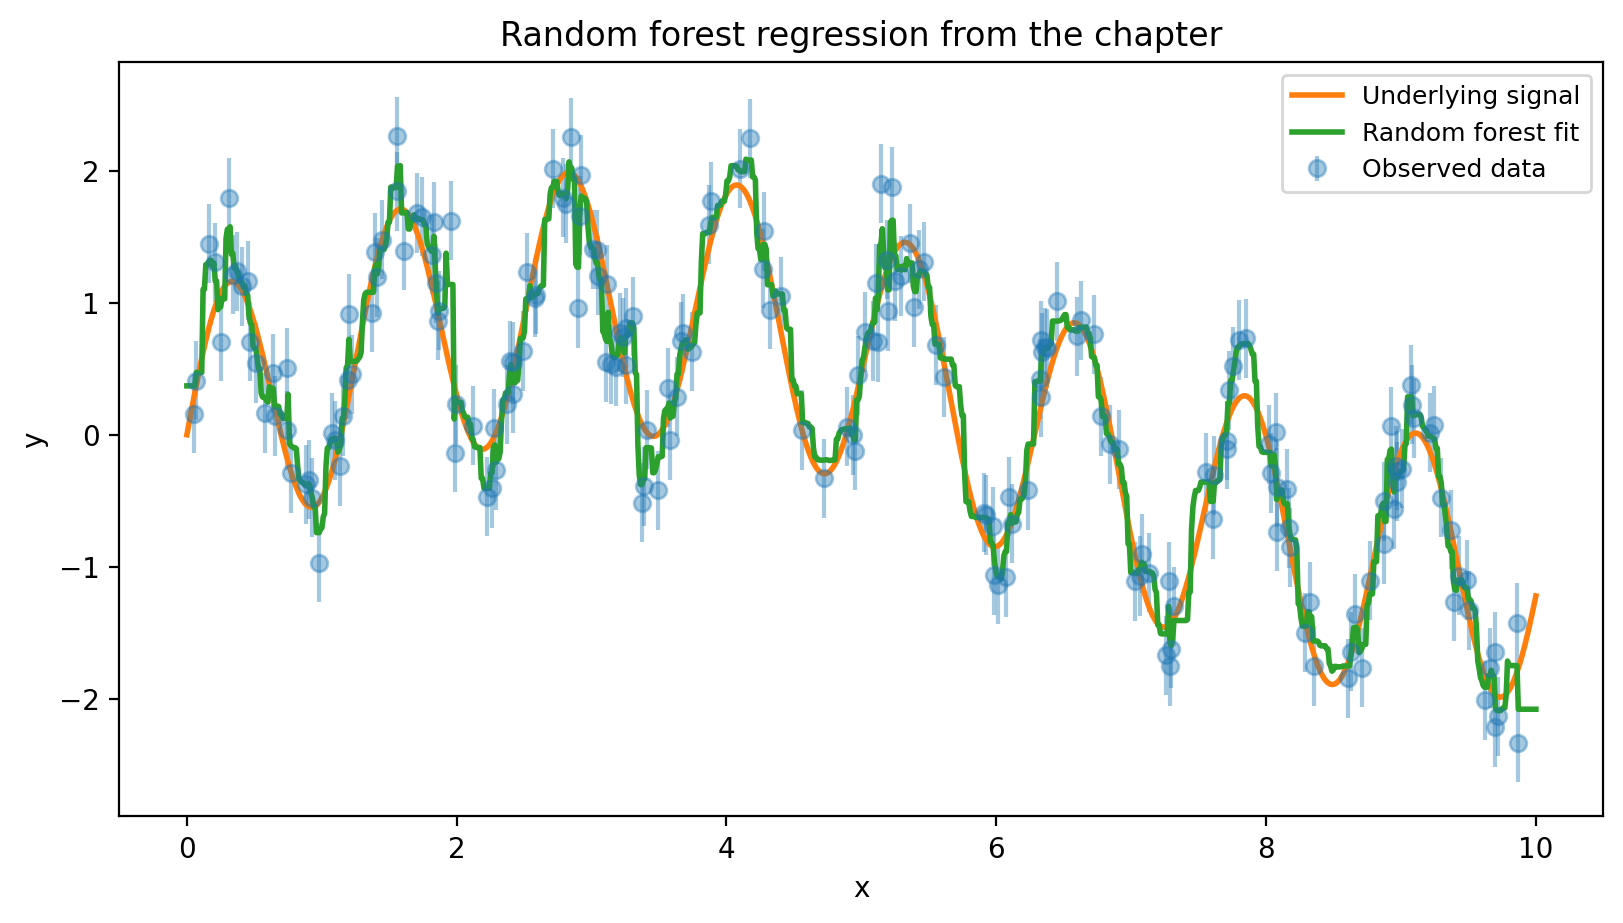
\includegraphics[height=0.63\textheight,keepaspectratio]{rf_regression.png}\par
\small In the handbook's two-frequency example,\\
a forest follows a noisy nonlinear signal without being told its formula.
\end{frame}

\begin{frame}{What does regression teach us?}
The chapter uses the signal
\[y = \sin(5x) + \sin(0.5x) + \varepsilon.\]
The forest can learn a flexible approximation from examples,\\
but its fitted curve can be jagged.
\vspace{0.7em}
\begin{itemize}
\item Classification forests combine votes.
\item Regression forests average predictions.
\item Neither automatically discovers the underlying scientific equation.
\end{itemize}
\end{frame}

\begin{frame}{A new task: recognize handwritten digits}
\centering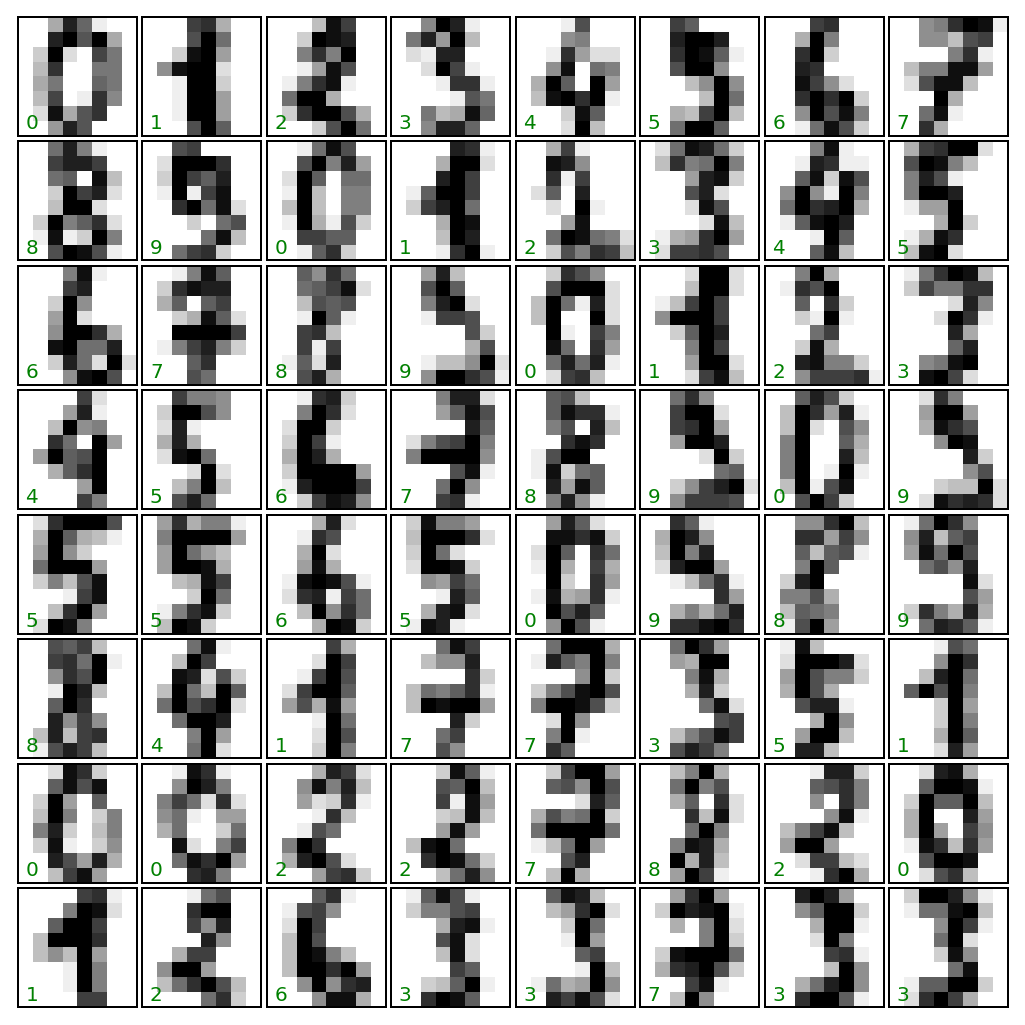
\includegraphics[height=0.61\textheight,keepaspectratio]{digits_grid.png}\par
\small Each image has 8$\times$8 pixels (64 features).\\
Can the forest recognize which digit it shows?
\end{frame}

\begin{frame}{Accuracy is not the whole story}
\textbf{Accuracy} tells us the share of all predictions that are correct.\\
It does not reveal which digit pairs are confused.
\par \vspace{0.8em}
A \textbf{confusion matrix} shows how actual and predicted classes compare.
\vspace{0.8em}
\begin{itemize}
\item The diagonal shows correct predictions.
\item Off-diagonal counts show specific mistakes.
\end{itemize}
\takeaway{A useful model report combines an overall metric with an error analysis.}
\end{frame}

\begin{frame}{Look for the mistakes}
\centering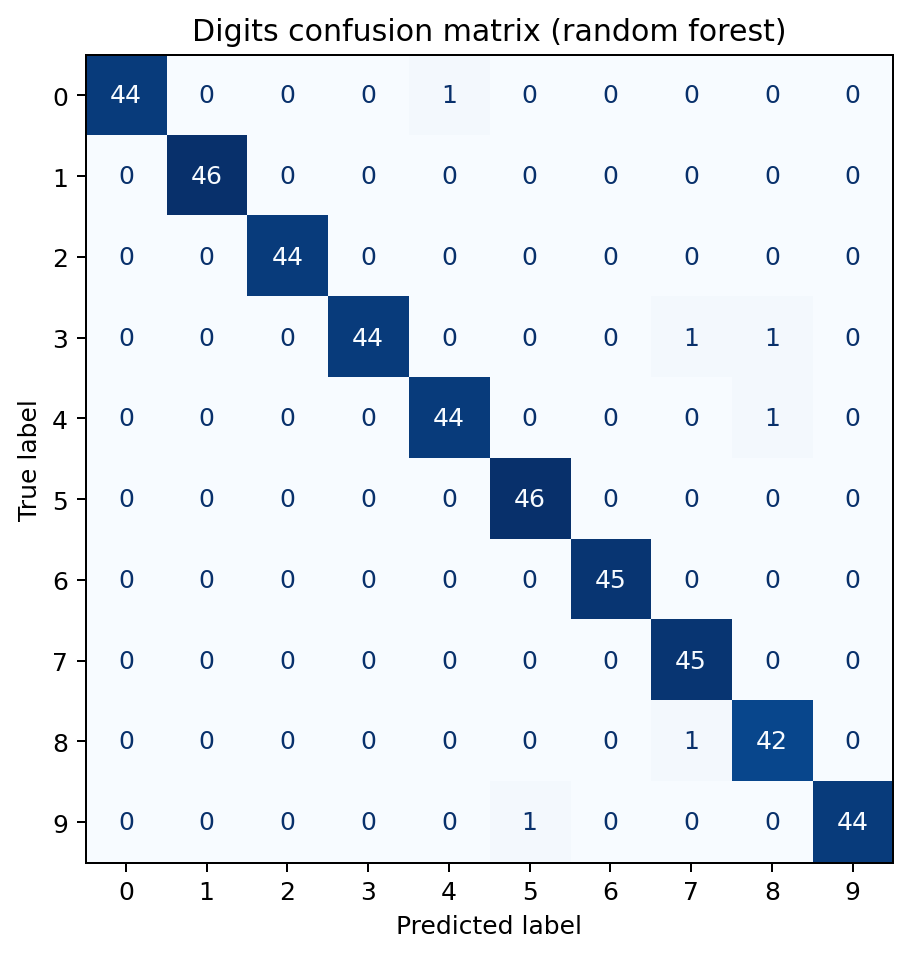
\includegraphics[height=0.65\textheight,keepaspectratio]{digits_confusion.png}\par
\small Find a cell outside the diagonal.\\
Which true digit was predicted as which other digit?
\end{frame}

\begin{frame}{Which claim is more defensible?}
\textbf{Claim A:} A random forest is always better than a single tree.
\par \vspace{1.2em}
\textbf{Claim B:} A random forest may generalize better, but the choice depends on the data, the evidence, and the need for interpretability.
\par 
\activity{Choose a claim; provide one reason and one piece of evidence you would want (3 min).}
\end{frame}

\begin{frame}{Your final in-class assignment}
\textbf{Question:} Should we use a decision tree or a random forest to classify the handbook's handwritten digits?
\par \vspace{1em}
\textbf{Deliverable:} One runnable notebook, plus a 150--250 word recommendation inside it.
\par \vspace{1em}
\textbf{Expectation:} Make a fair comparison, interpret the mistakes, and defend a choice.
\par \vspace{.5em}
\takeaway{Use the held-out test set for your final comparison, not for repeated model tuning.}
\end{frame}

\begin{frame}{Assignment: what to include}
\begin{enumerate}
\item Load \texttt{load\_digits()} and describe the data.
\item Use one stratified 75/25 split (\texttt{random\_state=0}).
\item Fit a tree and a forest on the same training set.
\item Report test \textbf{accuracy}, \textbf{macro-F1}, and a \textbf{confusion matrix} for each.
\item Identify one important error pattern or tradeoff.
\item Recommend one model and acknowledge one limitation.
\end{enumerate}
\end{frame}

\begin{frame}[fragile]{Start your notebook here}
\begin{lstlisting}
from sklearn.datasets import load_digits
from sklearn.model_selection import train_test_split
from sklearn.tree import DecisionTreeClassifier
from sklearn.ensemble import RandomForestClassifier
from sklearn.metrics import (accuracy_score, f1_score,
                             confusion_matrix)

X, y = load_digits(return_X_y=True)
Xtr, Xte, ytr, yte = train_test_split(
    X, y, test_size=.25, stratify=y, random_state=0)

# TODO: fit both models, predict, and compare
# TODO: report accuracy, macro-F1, confusion matrices
# TODO: recommend a model and state one limitation
\end{lstlisting}
\end{frame}

\begin{frame}{A simple plan for the class period}
\begin{itemize}
\item \textbf{0--5 min:} Inspect the data and predict the outcome.
\item \textbf{5--15 min:} Fit the two models.
\item \textbf{15--25 min:} Compute metrics and study errors.
\item \textbf{25--35 min:} Write the recommendation.
\item \textbf{35--40 min:} Exchange notebooks for peer review.
\end{itemize}
\takeaway{Prioritize a reproducible, well-explained comparison over visual polish.}
\end{frame}

\begin{frame}{Holistic rubric: one score from 0 to 4}
\small
\begin{description}
\setlength\itemsep{0.7em}
\item[4 --- Excellent] Fair, reproducible comparison; insightful error analysis; convincing recommendation and meaningful limitation.
\item[3 --- Proficient] Both models compared correctly; reasonable recommendation; minor gaps in explanation or reproducibility.
\item[2 --- Developing] Basic comparison present, but important gaps in evaluation or reasoning.
\item[1 --- Beginning] Incomplete or substantially flawed comparison, with little useful interpretation.
\item[0 --- No evidence] No assessable comparison submitted.
\end{description}
\vfill
\normalsize\textbf{Score the whole notebook, not separate checklist items.}
\end{frame}

\begin{frame}{Peer review and final reflection}
Ask a peer:
\begin{itemize}
\item Does the notebook run from top to bottom?
\item Are both models evaluated on the same held-out data?
\item Does the recommendation match the evidence?
\item Which rubric score best describes the whole submission?
\end{itemize}
\activity{Complete: ``I would choose \ldots\ because \ldots\ . The strongest evidence is \ldots\ . My biggest uncertainty is \ldots\ .''}
\end{frame}

\begin{frame}{}
A decision tree makes predictions through a series of questions.\par\medskip
A random forest builds many different trees and combines their predictions.\par\medskip
Neither model is automatically best: \textbf{the right choice depends on fair evaluation and the task.}
\end{frame}
\end{document}